\documentclass[a4paper,10pt,twoside]{article}
\usepackage[utf8]{inputenc}	% Text coding
\usepackage[T1]{fontenc}
\usepackage{lmodern}
\usepackage[czech]{babel}
\usepackage{epsfig}
\usepackage{amsfonts,amsmath,amssymb}
\usepackage{graphicx}
\usepackage[unicode]{hyperref}
\usepackage{indentfirst}
\usepackage{fancyhdr}
\usepackage{xifthen}
\usepackage{amsthm,thmtools}
\usepackage{bold-extra}
\usepackage[dvipsnames]{xcolor}
\usepackage[subrefformat=simple,labelformat=simple]{subcaption} % Instead of subfigure
\usepackage{listings}
\usepackage{comment}
\usepackage{titlesec}
\usepackage{underscore}
\usepackage{makecell}       % Šířky čar v tabulkách

% Page size
\addtolength{\topmargin}{-1cm} %\addtolength{\textheight}{-10cm}
\addtolength{\textwidth}{3cm} 
\addtolength{\textheight}{4cm} % Width and height of the text
\addtolength{\voffset}{-1cm} % Top margin
\addtolength{\hoffset}{-1cm}
\setlength{\headheight}{15pt}

\DeclareMathOperator{\e}{e}

\def\vector#1{\boldsymbol{#1}}								% Vector
\renewcommand{\d}{\mathrm{d}}
\newcommand{\derivative}[3][]{\ifthenelse{\isempty{#1}}	    % Normal derivative
	{\frac{\d{#2}}{\d{#3}}}
	{\frac{\d^{#1}{#2}}{\d{#3}^{#1}}}
}
\newcommand{\im}{\mathrm{i}}

\def\makematrix#1{\begin{pmatrix}#1\end{pmatrix}}       % Matrix
\def\abs#1{\left|#1\right|}
\def\probability#1{\mathrm{Pr}\left[#1\right]}
\def\expectation#1{\mathrm{E}\left[#1\right]}
\def\dispersion#1{\sigma_{#1}^{2}}
\def\c{,\!}

\def\code#1{\textnormal{\texttt{#1}}}
\def\file#1{\textnormal{\textbf{\texttt{#1}}}}
\def\ghfile#1#2{\textnormal{\textbf{\texttt{\href{https://github.com/PavelStransky/PCInPhysics2021/blob/main/#1#2}{#2}}}}}

\def\abbreviation#1{\textnormal{\textsc{#1}}}

\begin{document}

\section*{Zápočtová práce 18.5.2023}
\subsection*{Faradayova klec}
Uvažujte dva rovnoběžné dráty v rovině (kondenzátor), mezi kterými je elektrické napětí $U=\varphi_{2}-\varphi_{1}$.
Do prostoru mezi dráty je navíc vložena \emph{nenabitá} uzavřená klec z vodivého materiálu.
Klec se elektrod nedotýká.
\begin{center}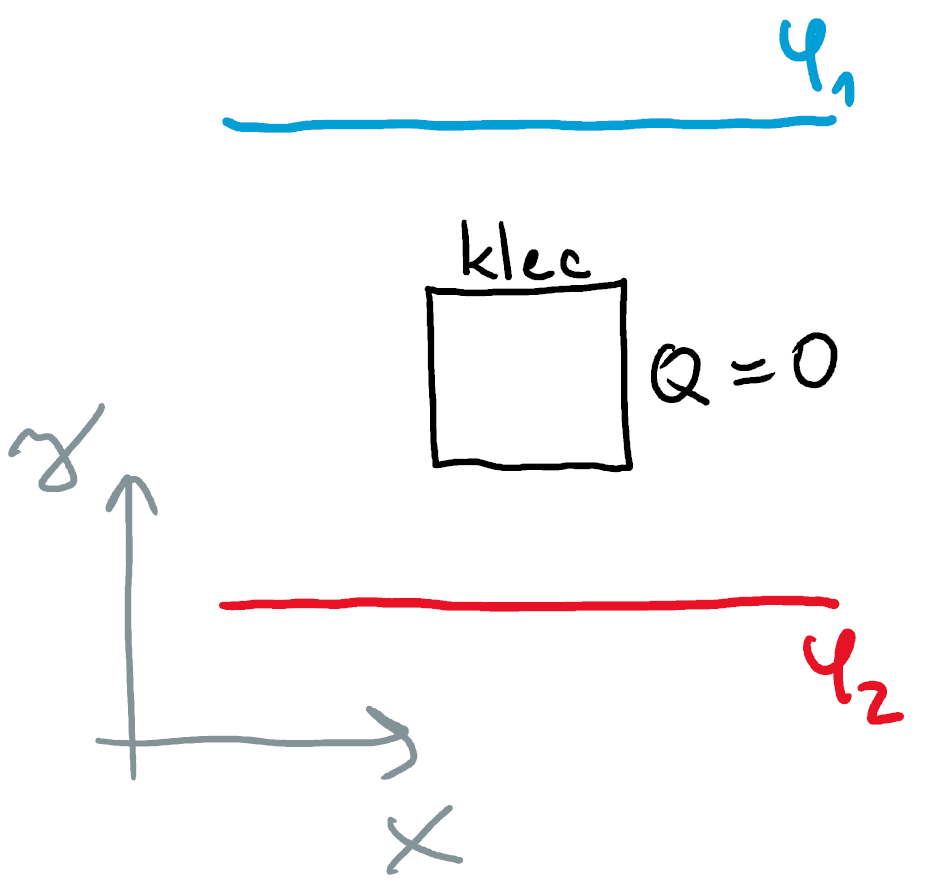
\includegraphics[width=0.3\linewidth]{klec.png}\end{center}

\begin{itemize}
    \item\emph{(2 body)} Vyřešte numericky 2D Laplaceovu rovnici elektrostatického pole
    \begin{equation*}
        \Delta\varphi=0
    \end{equation*}
    pro kondenzátor bez vložené klece.

    \item\emph{(1 bod)} Vykreslete graf (například konturový graf nebo čárový graf pro nějakou zvolenou hodnotu souřadnice $x$) potenciálu mezi elektrodami kondenzátoru.
    
    \item\emph{(3 body)} Vyřešte 2D Laplaceovu rovnici pro případ, kdy mezi elektrody vložíte vodivou klec.
    
    \item\emph{(1 bod)} Ukažte, že uvnitř klece je potenciál konstantní (a tedy nulová intenzita elektrostatického pole, $\vector{E}=-\nabla\varphi=0$).

	\item\emph{(3 body)} Klec se po vložení do elektrostatického pole polarizuje. 
    Pomocí Poissonovy rovnice
    \begin{equation*}
        \Delta\varphi=-\frac{\rho}{\epsilon_{0}},
    \end{equation*}
    kde $\epsilon_{0}$ je permitivita vakua, spočítejte hustotu náboje na povrchu klece $\rho=\rho(x,y)$ a celkový náboj klece
    \begin{equation*}
        Q=\int_{l=\text{klec}}\rho(x,y)\d l.
    \end{equation*}

    \item\emph{(3 body)} Program upravte tak, aby řešení odpovídalo zadání, tj. aby celkový náboj klece byl $Q=0$.

    \item\emph{(1 bod)} Vykreslete graf potenciálu mezi elektrodami kondenzátoru s vloženou nenabitou klecí.
\end{itemize}

Řešte numericky na mříži o velikosti alespoň $40\times40$ bodů.
Jednotky, potenciály $\varphi_{1}$ a $\varphi_{2}$ a přesný tvar a velikost klece zvolte dle vlastního uvážení a invence (nijak to neovlivní hodnocení). 
Vypracovaný úkol odešlete na e-mailovou adresu \href{mailto:pcfyzika@pavelstransky.cz}{pcfyzika@pavelstransky.cz} nebo jinak adekvátně předejte do konce cvičení, tj. do 16:20.


\subsubsection*{Hodnocení zápočtové práce a výsledná známka}
Za tuto práci lze získat maximálně 14 bodů.
K bodům za práci budou přičteny body za domácí úkoly, a to tak, že 
\includegraphics[width=0.3cm]{ano.png}~$\mapsto3$ body, 
\includegraphics[width=0.3cm]{maybe_bw.png}~$\mapsto1\frac{1}{2}$ bodu.
Výsledná známka bude určena na základě následujícího klíče ($b$ je celkový získaný počet bodů):
\begin{enumerate}
	\item (výborně) \emph{$b\geq12$ bodů}
	\item (velmi dobře) \emph{$9\leq b<12$ bodů}
	\item (dobře) \emph{$7\leq b<9$ bodů}
\end{enumerate}

\end{document}